\begin{titlepage}
\vspace{-10mm}
\begin{center}
\begin{tabular}{c}
\textup {\LARGE CZECH TECHNICAL UNIVERSITY}\\
\hline
\end{tabular}
\end{center}
\begin{center}
\vspace{-3mm}
\textup {\large FACULTY OF CIVIL ENGINEERING}
\vspace{20mm}\end{center}
\begin{figure}[h]
\begin{center}
%\includegraphics{PS/lev.ps}
\end{center}
\end{figure}
\begin{center}
\vspace{-3mm}
\begin{center}
\textup {\large DEPARTMENT OF STRUCTURAL MECHANICS}\\
\end{center}
\vspace{25mm}
\textrm {\Huge TRFEL}\\
\vspace{20mm}
\textrm {\LARGE Finite ELement Method for Transport Problems}\\
\vspace{60mm}
{\Large \bf Prague, 2002 - 2003}
\end{center}
\end{titlepage}
%%%%%%%%%%%%%%%%%%%%%%%%%%%%%%%%%%%%%%%%%%%%%%%%%%%%%%%%
%%%%%%%%%%%%%%%%%%%%%%%%%%%%%%%%%%%%%%%%%%%%%%%%%%%%%%%%
%%%%%%%%%%%%%%%%%%%%%%%%%%%%%%%%%%%%%%%%%%%%%%%%%%%%%%%%
%%%%%%%%%%%%%%%%%%%%%%%%%%%%%%%%%%%%%%%%%%%%%%%%%%%%%%%%

\newpage
\begin{center}
{\huge \bf Acknowledgments}
\end{center}
\vspace{30mm}
{\it Financial support for this work was provided by the EU Project ``MAECENAS''}




%%%%%%%%%%%%%%%%%%%%%%%%%%%%%%%%%%%%%%%%%%%%%%%%%%%%%%%%
%%%%%%%%%%%%%%%%%%%%%%%%%%%%%%%%%%%%%%%%%%%%%%%%%%%%%%%%
%%%%%%%%%%%%%%%%%%%%%%%%%%%%%%%%%%%%%%%%%%%%%%%%%%%%%%%%
%%%%%%%%%%%%%%%%%%%%%%%%%%%%%%%%%%%%%%%%%%%%%%%%%%%%%%%%
\chapter{Introduction}

Analysis of complicated mechanical structures frequently leads to coupled systems of equations involving 
different physical fields. Some of these fields are of vector type while others, e.g. temperature, concentration, 
electric potential, etc., remain scalar. Most of them are governed by partial differential equations, generally 
resulting from conservation principles.

The governing equations, including the above mentioned scalar fields, can be linear or nonlinear. In problems 
of practical importance, however, substantial differences in temperatures, concentrations, electric potentials, etc., 
cause the dependence of material properties on required physical field. As a result, the system of governing equation 
becomes nonlinear and special algorithms are required to obtain solutions.

Major numerical techniques are finite differences method, finite elements method (FEM) 
and boundary elements method.

Application of FEM to linear or nonlinear problems requires certain modifications and special algorithms. 
...

TRFEL is a part of SIFEL (SImple Finite ELement) system dealing with
transport problems. The aim of TRFEL is to solve heat and moisture transfer in porous medium 
using modern theories and new materials models and approaches.
...

The finite element method is discussed and illustrated on a stationary linear diffusion problem and on 
a nonstationary linear diffusion problem in the {\bf Theoretical part I}.
Derivation of differential equations is shown and then the numerical solution using FEM follows.

...

...

...

...

Customary matrix notation is used throughout the text. Matrices are denoted by uppercase 
boldface italic letters, e.g., $\tenss{A,B}$ etc. Conversely, lowercase boldface italic letters 
stand for vectors $\tenss{\sigma,r}$ etc.

In the {\bf part II}, {\bf Computer implementation}, ... 

